%----PrefaceImport----%
\documentclass{article}
\usepackage{fancyhdr}
\usepackage[a4paper,margin=1in,headsep=25pt]{geometry}
\usepackage{lipsum,hyperref}
\usepackage{enumerate,fullpage,proof}
\usepackage[fontsize=12pt]{fontsize}
\usepackage{amsmath,amscd,amsbsy,amssymb,latexsym,url,bm,amsthm}
\usepackage{epsfig,graphicx,subfigure}
\usepackage{listings}
\usepackage[usenames]{xcolor}

\newtheorem{thm}{Theorem}
\newtheorem{lemma}[thm]{Lemma}

\pagestyle{fancy}
\pagenumbering{Alph}
\setlength{\headheight}{36.0pt}
\headsep = 25pt
\fancyhf{}
\lhead{CSE 4392/5369}
\rhead{Homework 6: Neural Network Basics}
\lfoot{2026 Kenny Zhu}
%----Documentation----%
\begin{document}

\title{CSE 4392/5369 Special Topic: Natural Language Processing}
\author{Homework 6 - Spring 2026}
\date{Due Date: March 2, 2026, 11:59 PM}
\maketitle
\thispagestyle{fancy}

%----Homeworks----%

Welcome to our exploration of Neural Network Basics. This assignment takes you on a journey from understanding the core principles of neural network architecture to hands-on experiences, such as manually calculating gradients for parameter optimization. We'll begin by solidifying your grasp of the basics and progress to the heart of the matter – computing gradients and formulating the update equation.

\section*{Problem 1 - 40\%}
In this task, you are provided with a simple fully connected neural network represented by figure~\ref*{fig:nn}. Your objective is to delve into the mathematical intricacies of backpropagation and calculate the gradients for each parameter in the network. The neural network consists of interconnected layers, and your task involves understanding the chain rule and applying it meticulously to determine how changes in each parameter affect the overall loss.
\begin{figure}[h]
    \centering
    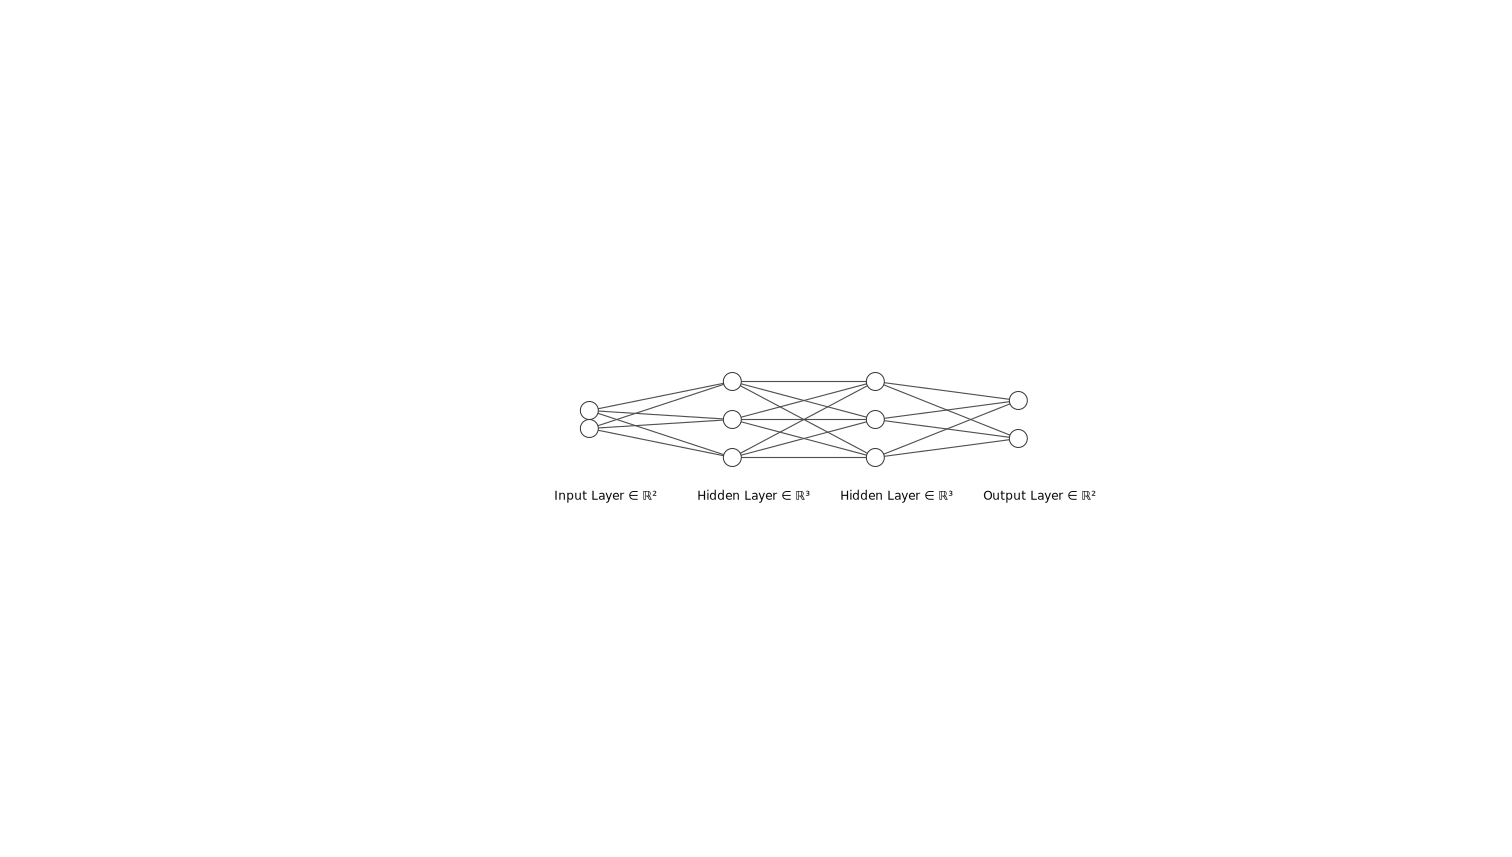
\includegraphics[width=1\textwidth]{hw6nn.png}
    \caption{A Simple Neural Network Architecture}
    \label{fig:nn}
\end{figure}
\newline
To guide your calculations, the feed forward procedure can be formulated as the equation shown below, consider the architecture of the neural network, paying special attention to \textbf{activation functions} $\tanh(\cdot)$, \textbf{weight matrices} $\mathbf{W}_{1}, \mathbf{W}_{2}, \mathbf{w}$, and \textbf{biases} $\mathbf{b}_{1}, \mathbf{b}_{2}, b$ and calculate these parameters' gradient on the cross entropy loss function. Once you've successfully computed the gradients, your next step is to \textbf{articulate the update equation} for each parameter. This process is fundamental for optimizing the network's performance through gradient descent.

$$Input: \mathbf{x}$$
$$\mathbf{h}_{1}=\tanh(\mathbf{W}_{1}\mathbf{x}+\mathbf{b}_{1})$$
$$\mathbf{h}_{2}=\tanh(\mathbf{W}_{2}\mathbf{h}_{1}+\mathbf{b}_{2})$$
$$\mathbf{y}=\sigma(\mathbf{w}^{\mathbf{T}}\mathbf{h}_{2}+b)$$
$$\mathcal{L}(\mathbf{y}, \mathbf{y}^*) = -y^*\log y - (1-y^*)\log (1-y) $$
\section*{Problem 2 - 60\%}
In this problem, you will leverage your understanding of neural network fundamentals to build a simple fully connected neural network for classifying MBTI (Myers-Briggs Type Indicator) personality types based on preprocessed posts.
\\
\newline
\textbf{dataset}: \href{https://drive.google.com/file/d/1CHuGdZKJJRl_IRdxa3MBv4SqEJVUhK73/view?usp=sharing}{MBTI 500.csv}
\\
\textbf{columns}:
\begin{itemize}
    \item \textbf{posts}: Equal-sized posts with 500 words per sample.
    \item \textbf{type}: MBTI personality types indicating differing psychological preferences.
\end{itemize}
\textbf{instructions}:
\begin{enumerate}
    \item \textbf{Dataset Exploration:}
        \begin{itemize}
            \item Load the provided CSV file (\textbf{MBTI500.csv}) into your preferred programming environment (e.g., Python with pandas).
        \end{itemize}
    \item \textbf{Data Preprocessing:}
        \begin{itemize}
            \item Decide whether to perform a 4-way classification (based on dichotomies) or a 16-way classification (considering each personality type independently). Your decision will guide how you preprocess the type column.
        \end{itemize}
    \item \textbf{Feature Extraction:}
        \begin{itemize}
            \item Utilize existing libraries (e.g., scikit-learn) to extract features from the posts. You may choose methods like TF-IDF or word embeddings for this purpose.
        \end{itemize}
    \item \textbf{Neural Network Construction:}
        \begin{itemize}
            \item Build a simple fully connected neural network \textbf{from scratch} (\textcolor{red}{please do not use exist neural network libraries}), adhering to the specifications discussed in the lecture and utilizing the results in Problem 1.
        \end{itemize}
    \item \textbf{Training:}
        \begin{itemize}
            \item Implement the backpropagation algorithm to train your neural network. Set hyperparameters such as learning rate, batch size, and epochs.
        \end{itemize}
    \item \textbf{Evaluation:}
        \begin{itemize}
            \item Use k-fold cross-validation to evaluate the performance of your model. Analyze metrics such as accuracy, precision, recall, and F1 score.
        \end{itemize}
    \item \textbf{Documentation:}
        \begin{itemize}
            \item Create a report detailing your approach, including decisions made during data preprocessing, feature extraction, and network architecture. Provide insights into your model's performance and discuss any challenges faced.
        \end{itemize}
    \item \textbf{Attach your codes and report.}
\end{enumerate}


\vspace{0.8em}
\noindent{\color{red}\footnotesize
\textbf{Submission Format:}
Submit one zip file via Canvas containing only
the \texttt{.pdf} version of your homework (typed submissions are preferred;
scanned images must be readable), the corresponding
source files, and a \texttt{README} file describing how to run the code.
The zip file must be named
\texttt{lastname\_studentID\_hw6.zip}.
}



\end{document}
